\documentclass[t, screen, aspectratio=43]{beamer}
\usepackage[T1]{fontenc}
\usepackage[utf8]{inputenc}
\usepackage{epsf}
\usepackage{graphicx}
\usepackage{geometry}
\usepackage{tabularx}
\usepackage[table]{colortbl}
% Use the NTNU-temaet for beamer 
% \usetheme[style=ntnu|simple|vertical|horizontal, 
%     language=bm|nn|en, 
%     smalltitle, 
%     city=all|trondheim|alesund|gjovik]{ntnu2017}
\usetheme[style=helvet,language=en]{ntnu2017}

\usepackage[english]{babel}
\usepackage[style=numeric,backend=biber,natbib=false,sorting=none]{biblatex}

\title[Short title]{Ultra-Low Power PLL for Wake-up Receiver Applications}
\subtitle{Specialization Project}
\author[C Nielsen]{Cole Nielsen}
\institute[NTNU]{Department of Electronic Systems, NTNU}
\date{30 August 2019}
%\date{} % To have an empty date

\addbibresource{example.bib} % Add bibliography database

% Set the reference style to numeric.
% See here: http://tex.stackexchange.com/questions/68080/beamer-bibliography-icon
\setbeamertemplate{bibliography item}[text] 

% Set bibliography fonts to a small size.
\renewcommand*{\bibfont}{\footnotesize}

\begin{document}

\begin{frame}
	\titlepage%
\end{frame}

% Alternatively, special title page command to get a different background
% \ntnutitlepage

% #############################################################################
% Motivation
% #############################################################################

\begin{frame}
	\frametitle{Motivation}
	\begin{block}{Wireless Sensor Networks (WSNs) and IoT}
		\begin{itemize}
			\footnotesize
			\item WSNs require ultra-low power circuits. A sensor should last for many years (>5) on a coin cell battery.
			\item With the below $P_{avg}$ values, a CR2032 cell with 0.6 Wh capacity will last:
			\begin{itemize}
				\scriptsize
				\item 1 $\mu$W $\rightarrow$ 70 years
				\item 10 $\mu$W $\rightarrow$ 7 years
				\item 100 $\mu$W $\rightarrow$ 0.7 years
			\end{itemize} 
			\item To save power, run devices with low duty cycle; activate remotely using wake up receiver (WuRx).
			\begin{itemize}
				\scriptsize
				\item For 5 years of life, using 10\% of battery energy for the WuRx, \textbf{$P_{WURX}$ < 1.4 $\mu$W} on average is required.
			\end{itemize} 
			\item Main challenge for receiver is low power LO synthesis.
			\begin{itemize}
				\scriptsize
				\item Synthesizer-free approaches (OOK receiver) lack robustness.
				\item Advanced modulation schemes are too demanding with phase noise (PN).
				\item Best option is FSK, using low power synthesizer with loose PN requirements to meet power target.
			\end{itemize} 
		\end{itemize}    
	\end{block}
\end{frame}

% #############################################################################
% State of Art
% #############################################################################

\begin{frame}
	\frametitle{State of the Art}
	\begin{block}{Wake Up Receivers}
		\footnotesize
		Performance averages based on sampling of 15 works published in IEEE:
		\scriptsize
		\vspace{-1em}
		\begin{table}[htb!]
			\tiny
			\centering
			\def\arraystretch{1.5}		
			\setlength\arrayrulewidth{0.75pt}
			\setlength{\tabcolsep}{1em} % for the horizontal padding
			\begin{tabular}{|l|l|l|l|l|l|l|l|}
				\hline 
				\rule[-1ex]{0pt}{2.5ex} \cellcolor{gray!40}\textbf{Group} & \cellcolor{gray!40}\textbf{Count} & \cellcolor{gray!40}\textbf{Power [$\mu$W] }& \cellcolor{gray!40}\textbf{Freq [MHz]} & \cellcolor{gray!40}\textbf{RF BW [MHz]}& \cellcolor{gray!40}\textbf{Bitrate [kbps]}& \cellcolor{gray!40}\textbf{BER }& \cellcolor{gray!40}\textbf{Sens. [dBm]}\\ 
				\hline 
				\rule[-1ex]{0pt}{2.5ex} \textbf{All} & 15 & 96 & 1400 & 1.2 & 52 & 3e-3 & -66\\ 
				\hline 
				\rule[-1ex]{0pt}{2.5ex} \textbf{800/900M} & 6 & 138 & 887 & 0.95 & 15 & 4e-3 & -68\\ 
				\hline 
				\rule[-1ex]{0pt}{2.5ex} \textbf{All 2.4G} & 6 & 81 & 2400 & 2 & 60 & 2.8e-3 & -67\\ 
				\hline 
				\rule[-1ex]{0pt}{2.5ex} \textbf{2.4G FSK} & 2 & 190 & 2400 & 1.5 & 98 & 1e-3 & -69\\ 
				\hline 
				\rule[-1ex]{0pt}{2.5ex} \textbf{2.4G OOK} & 4 & 27 & 2400 & 2.5 & 41.5 & 4e-3 & -66\\ 
				\hline 
			\end{tabular} 
			% \caption{Assigned specifications for branch line hybrid design.}
			% \label{asgn_specs}
		\end{table}   
		\begin{itemize}
			\footnotesize
			\item State of art of 2.4G WuRx:
			\begin{itemize}
				\item Active Power $\leq$ 100 $\mu$W
				\item RF BW $\approx$ 1 MHz
				\item Sensitivity = -70 dBm (BER 1e-3)
				\item Data Rate = 100 kbps
			\end{itemize}
		\end{itemize}

	\end{block}

\end{frame}
% #############################################################################
% Project objectives
% #############################################################################

\begin{frame}
	\frametitle{Objective}
	\begin{block}{Synthesizer Goals}
		\begin{itemize}
			\footnotesize
			\item Design ultra-low-power frequency synthesizer to meet requirements for \textit{practical} wake up receivers.
			\begin{itemize}
				\footnotesize
				\item \textbf{$\leq$1 $\mu$W average consumption}
				\item Targeting \textbf{1\% duty cycle} for \textbf{$\leq$100 $\mu$W active power}.
				\begin{itemize}
					\item Fast locking to reduce on time/energy consumption.
				\end{itemize}
			\end{itemize} 
			\item Synthesis range within \textbf{2.4 GHz ISM band}.
			\item Enable \textbf{wake up call detection within 1s} with 1e-3 miss rate.
			\begin{itemize}
				\scriptsize
				\item Achievable with 250 kbps data, BER $\leq$ 1e-2, 1\% duty, 20\% wake up call Tx density.
				\item Assuming 32-symbol wake up call used for false-alarm robustness.
				\item High BER inherent due to high PN, expect many misses before sucess.  
				\item Use large FSK modulation index (m) to ease PN and power requirements. 
				\begin{itemize}
					\scriptsize
					\item m=2 $\rightarrow$ 2$\pi$ phase shift per symbol or $\pm$250 kHz frequency deviation.
					\item RMS Residual frequency modulation (RFM) of PLL should be $<<$ symbol frequency deviation to achieve desired BER.
					\item \textbf{RFM is derived from phase noise integration; use to constrain PLL PN.}
				\end{itemize}
			\end{itemize}      
		\end{itemize}
	\end{block}
\end{frame}

% #############################################################################
% Specification
% #############################################################################

\begin{frame}
	\frametitle{Specification}
	\begin{block}{Preliminary Performance Targets}
		\scriptsize
		\begin{table}[h!]
			\centering
			\def\arraystretch{1.5}		
			\setlength\arrayrulewidth{0.75pt}
			\setlength{\tabcolsep}{1em} % for the horizontal padding
			\begin{tabular}{|l|r|l|l|}
				\hline 
				\rule[-1ex]{0pt}{2.5ex} \cellcolor{gray!40}\textbf{Parameter} & \cellcolor{gray!40}\textbf{Value} & \cellcolor{gray!40}\textbf{Unit }& \cellcolor{gray!40}\textbf{Notes}\\ 
				\hline 
				\rule[-1ex]{0pt}{2.5ex} \textbf{Frequency}  & 2.4-2.4835 & GHz & 2.4G ISM Band\\ 
				\hline 
				\rule[-1ex]{0pt}{2.5ex} \textbf{Ref. frequency} & 16 & MHz & Yields 6 channels \\ 
				\hline 
				\rule[-1ex]{0pt}{2.5ex} \textbf{Power} & $\leq$ 100  &$\mu$W & \\ 
				\hline 
				\rule[-1ex]{0pt}{2.5ex} \textbf{Residual FM} & $\leq$ 107  &kHz$_{RMS}$ & BER $\leq$ 1e-2, $f_{dev}$=$\pm$250 KHz\\ 
				\hline 
				\rule[-1ex]{0pt}{2.5ex} \textbf{Initial Lock Time} & $\leq$ 50 & $\mu$s & Upon cold start \\ 
				\hline 
				\rule[-1ex]{0pt}{2.5ex} \textbf{Re-lock Time} & $\leq$ 5 & $\mu$s & Coming out of standby \\ 
				\hline 
				\rule[-1ex]{0pt}{2.5ex} \textbf{Bandwidth} & 100 & kHz & (nominally), tunable \\ 
				\hline 
			\end{tabular} 
			% \caption{Assigned specifications for branch line hybrid design.}
			% \label{asgn_specs}
		\end{table}   
		Additionally: PLL output should support IQ sampling at LO frequency.
	\end{block}    
\end{frame}

% #############################################################################
% Architecture - ideas
% #############################################################################

\begin{frame}
	\frametitle{Architecture}
	\begin{block}{Concept}
		\begin{itemize}
			\footnotesize
			\item Utilize \textbf{Digital PLL}.\@ 
			\begin{itemize}
				\footnotesize
				\item Inherent feedback helps with PVT variation (yield).
				\item Calibration easy in digital design, agains helps with PVT variation.
				\item Can store state when PLL idle, allowing for faster lock times coming out of standby.
			\end{itemize}       
		  \item Utilize low duty cycle to achieve power target.     
			\begin{itemize}
				\footnotesize
				\item Can exploit semi-frequent calibration to improve performance.
				\item Possibly can run PLL open loop when lock is achieved to save power.
			\end{itemize} 
		  \item Utilize oscillator running at 1/N subharmonic of target frequency.
			\begin{itemize}
				\footnotesize
				\item Use 2N phases in oscillator to achieve equivalent IQ sampling.
				\item Avoids having to run oscillator at 2x target frequency as done typically.
				\item 1/3 subharmonic operation should allow for dual mode 2.4G and 915M operation.
			\end{itemize} 
			\item Employ subsampling to reduce divider noise and TDC power?
		\end{itemize}
	\end{block}    

\end{frame}

% #############################################################################
% Architecture - block diagram
% #############################################################################

\begin{frame}
	\frametitle{Architecture}
	\begin{block}{Block Diagram}
		\center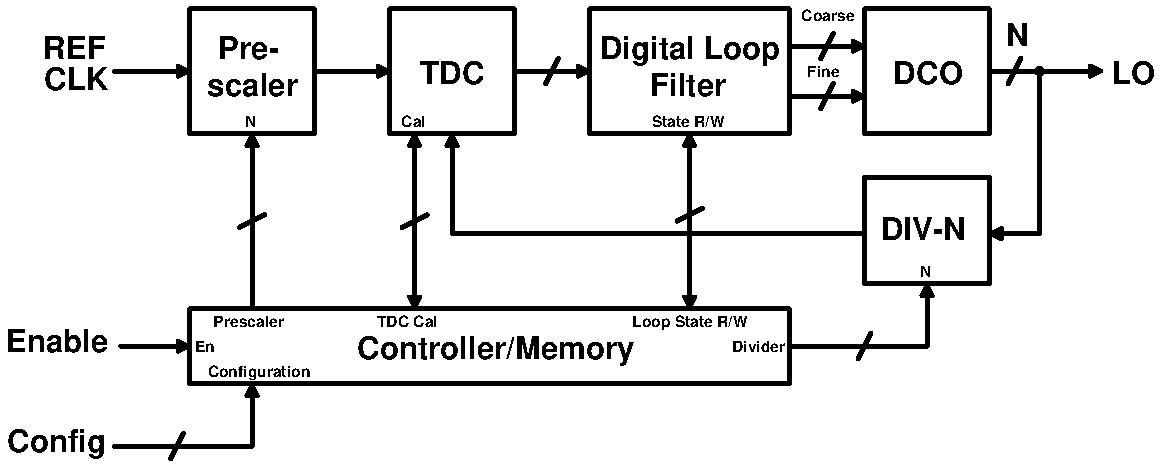
\includegraphics[width=0.75\textwidth, angle=0]{pll2.pdf}

		\end{block}
		\begin{block}{Power Targets}
		\begin{table}[htb!]
			\tiny
			\centering
			\def\arraystretch{1.5}		
			\setlength\arrayrulewidth{0.75pt}
			\setlength{\tabcolsep}{1em} % for the horizontal padding
			\begin{tabular}{|l|l|l|l|l|}
				\hline 
				\rule[-1ex]{0pt}{2.5ex} \cellcolor{gray!40}\textbf{DCO} & \cellcolor{gray!40}\textbf{TDC} & \cellcolor{gray!40}\textbf{Divider }& \cellcolor{gray!40}\textbf{Other} & \cellcolor{gray!40}\textbf{SUM} \\ 
				\hline 
				\rule[-1ex]{0pt}{2.5ex} 70 $\mu$W& 20 $\mu$W & 10 $\mu$W & $<<$ 1 $\mu$W & 100 $\mu$W\\ 
				\hline 
			\end{tabular} 
			% \caption{Assigned specifications for branch line hybrid design.}
			% \label{asgn_specs}
		\end{table}   
	\end{block}

\end{frame}

% #############################################################################
% State of Art
% #############################################################################

\begin{frame}
	\frametitle{State of the Art}
	\begin{block}{Sub 1-mW PLLS}
		\footnotesize Application is niche, so comparable PLLs hard to find.
		\vspace{-1em}
		\begin{table}[htb!]
			\tiny
			\centering
			\def\arraystretch{1.5}		
			\setlength\arrayrulewidth{0.75pt}
			\setlength{\tabcolsep}{1em} % for the horizontal padding
			\begin{tabular}{|l|l|l|l|l|l|l|l|}
				\hline 
				\rule[-1ex]{0pt}{2.5ex} \cellcolor{gray!40}\textbf{Type} & \cellcolor{gray!40}\textbf{P$_{PLL}$ [$\mu$W]}& \cellcolor{gray!40}\textbf{P$_{osc}$ [$\mu$W] }& \cellcolor{gray!40}\textbf{Freq [MHz]} & \cellcolor{gray!40}\textbf{PN@$\Delta f$ [dBc/Hz]}& \cellcolor{gray!40}\textbf{t$_{lock}$* [$\mu$s]}& \cellcolor{gray!40}\textbf{Osc. }& \cellcolor{gray!40}\textbf{Ref Freq}\\ 
				\hline 
				\rule[-1ex]{0pt}{2.5ex} \textbf{Dig. Frac-N} & 650 & 304 & 2400 & -110@0.5M & 15/4 & LC & 26M\\ 
				\hline 
				\rule[-1ex]{0pt}{2.5ex} \textbf{Ana. Int-N }& 680 & 510 & 2400 & -110@1M & 130/70 & LC & 1M\\ 
				\hline 
				\rule[-1ex]{0pt}{2.5ex} \textbf{Ana. Int-N} & 128 &  & 500 & -94@1M &  & Ring & 31.25M\\ 
				\hline 
				\rule[-1ex]{0pt}{2.5ex} \textbf{Ana. Int-N} & 570 &  & 800 & -92.6@0.1M & 200 & LC & 0.2M\\ 
				\hline 
				\rule[-1ex]{0pt}{2.5ex} \textbf{Dig. Frac-N} & 250 & 173 & 2448 &  & 22/1 & Ring & 9M\\ 
				\hline 
				\rule[-1ex]{0pt}{2.5ex} \textbf{Ana. Int-N} & 950 &  & 5500 & -106@1M &  & IL-LC & \\ 
				\hline 
			\end{tabular} 
			% \caption{Assigned specifications for branch line hybrid design.}
			% \label{asgn_specs}
		\end{table}  
		\tiny
		\vspace{-1em}
		*Initial lock time and relock time
		\begin{itemize}
			\scriptsize
			\item Power limited by oscillator type. Scaling of LC-oscillator limited by gain requirements for self-starting. LC does not scale to low enough power.
			\item Current state of art for minimum power will be with ring oscillator, on the order of 200 $\mu$W for total PLL consumption.
		\end{itemize}
	\end{block}

\end{frame}

% #############################################################################
% Physical limits
% #############################################################################

\begin{frame}
	\frametitle{Physical limits}
	\begin{block}{Ring Oscillator Phase Noise}
		\scriptsize
		Ring oscillator phase noise limit from "Minimum Achievable Phase Noise of RC Oscillators", Navid et al. 2005:
		\begin{equation}
			PN_{min}(\Delta f)= 10\log 10\left(\frac{7.33k_BT}{P}\left(\frac{f_0}{\Delta f}\right)^2\right)
		\end{equation}
		\vspace{-.8em}\\
		If $f_0$ = 2.4 GHz, P = 50 $\mu$W, $\Delta f$= 1 MHz, T = 293 K, $\rightarrow$ \textbf{PN$_{min}$ = -84.7 dBc/Hz} \\
		-- This limit applied to the below FOM comparison (FOM PN=165 dB):
		\vspace{-1.5em}
		\center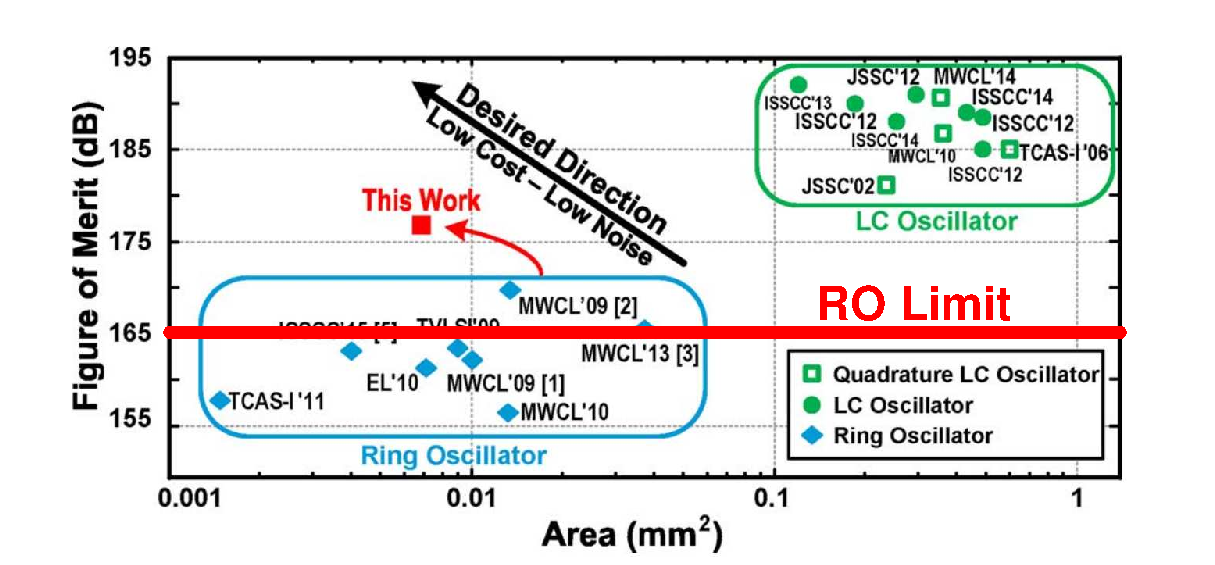
\includegraphics[width=0.75\textwidth, angle=0]{ro_perf.pdf}
	\end{block}
\end{frame}
% #############################################################################
% Project phases slide 1
% #############################################################################

\begin{frame}
	\frametitle{Project Phases}
	\begin{block}{Autumn 2019}
		\footnotesize
		\begin{itemize}
			\item System modeling and simulation.
			\begin{itemize}
				\footnotesize
				\item Learn PLL theory in detail
				\item Evaluate feasability of PLL architectures (counter, TDC-based)
				\item Determine requirements for TDC/DCO/Divider/logic (bits of resolution, accuracy etc) to meet PLL performance specifications.
				\item Determine digital logic for loop filter, validate stability and lock time performance.
			\end{itemize}
			\item Research ultra-low power circuit topologies to implement system components that will meet determined requirements.
			\item Translate component-level specifications into schematic-level circuit designs.
			\begin{itemize}
				\footnotesize
				\item Try, fail, try again until functional at schematic level.
				\begin{itemize}
					\footnotesize
					\item I expect the TDC to be difficult.
				\end{itemize}
			\end{itemize}      
		\end{itemize}
	\end{block}
\end{frame}

% #############################################################################
% Project phases slide 2
% #############################################################################


\begin{frame}
	\frametitle{Project Phases (continued)}
	\begin{block}{Spring 2020}
		\begin{itemize}
			\footnotesize
			\item Finalize schematic-level design.
			\item Estabilish thorough tests for PLL performance (automated?) to help in layout.
			\item Layout of PLL.
			\begin{itemize}
				\footnotesize
				\item Design iteration until design specs met.
				\item Probably very time consuming.
			\end{itemize}
			\item Full characterization/validation of design performance. 
			\begin{itemize}
				\footnotesize
				\item Comprehensive Corners/Monte-Carlo testing (time consuming??)
				\item More design iteration if new issues crop up...
			\end{itemize}
			\item Thesis paper writing.
		\end{itemize}
	\end{block}
\end{frame}


\begin{frame}
	\frametitle{Autumn Timeline}
	\begin{table}[htb!]
		\tiny
		\centering
		\def\arraystretch{1.5}		
		\setlength\arrayrulewidth{0.75pt}
		\setlength{\tabcolsep}{1em} % for the horizontal padding
		\begin{tabular}{|l|l|l|l|}
			\hline 
			\rule[-1ex]{0pt}{2.5ex} \cellcolor{gray!40}\textbf{Week Number} & \cellcolor{gray!40}\textbf{Dates} &\cellcolor{gray!40}\textbf{Tasks} & \cellcolor{gray!40}\textbf{Outcomes}\\ 
			\hline 
			\rule[-1ex]{0pt}{2.5ex} \textbf{36}& 2.9 - 8.9 & Review PLL Design & Refreshed Knowledge\\ 
			\hline 
			\rule[-1ex]{0pt}{2.5ex} \textbf{37}& 9.9 - 15.9 & Modeling/simulation (set up) & --\\ 
			\hline 
			\rule[-1ex]{0pt}{2.5ex} \textbf{38}& 16.9 - 22.9 & Modeling/simulation & TDC/DCO Requirements\\ 
			\hline 
			\rule[-1ex]{0pt}{2.5ex} \textbf{39}& 23.9 - 29.9& Modeling/simulation& Loop Filter/Digital Algorithms\\ 
			\hline 
			\rule[-1ex]{0pt}{2.5ex} \textbf{40}& 30.9 - 6.10& Modeling/simulation& Ideal (ahdlLib?) implementation in Cadence of PLL\\ 
			\hline 
			\rule[-1ex]{0pt}{2.5ex} \textbf{41}& 7.10 - 13.10& Circuit Research & DCO/Divider topologies\\ 
			\hline 
			\rule[-1ex]{0pt}{2.5ex} \textbf{42}& 14.10 - 20.10& Circuit Research & TDC/other topologies\\ 
			\hline 
			\rule[-1ex]{0pt}{2.5ex} \textbf{43}& 21.10 - 27.10& Circuit Implementation& Digital logic (schematic)\\ 
			\hline 
			\rule[-1ex]{0pt}{2.5ex} \textbf{44}& 28.10 - 3.11& Circuit Implementation& DCO (schematic)\\ 
			\hline 
			\rule[-1ex]{0pt}{2.5ex} \textbf{45}& 4.11 - 10.11& Circuit Implementation& Divider/other (schematic)\\ 
			\hline 
			\rule[-1ex]{0pt}{2.5ex} \textbf{46}& 11.11 - 17.11& Circuit Implementation (TDC)& \\ 
			\hline 
			\rule[-1ex]{0pt}{2.5ex} \textbf{47}& 18.11 - 24.11& Circuit Implementation (TDC)& TDC (schematic)\\ 
			\hline 
			\rule[-1ex]{0pt}{2.5ex} \textbf{48}& 25.11 - 1.12& Full Circuit testing & Testbenches, find bugs, design fixes\\ 
			\hline 
			\rule[-1ex]{0pt}{2.5ex} \textbf{49}& 2.12 - 8.12& Full Circuit testing& Design Fixes/iteration\\ 
			\hline 
			\rule[-1ex]{0pt}{2.5ex} \textbf{50}& 9.12 - 15.12& --& --\\ 
			\hline 
		\end{tabular} 
		% \caption{Assigned specifications for branch line hybrid design.}
		% \label{asgn_specs}
	\end{table}   
\end{frame}

\end{document}
